\section{Лекция 1 24.02.25. Численные методы решения нелинейных уравнений и систем}
\subsection{Постановка задачи}
Пусть $\mathbf{x} = \begin{pmatrix} 
x_1    \\ 
x_2    \\ 
\vdots \\ 
x_n    
\end{pmatrix} \in \mathbb{R}^n, F \in C(\mathbb{R}^n).
$
Дано уравнение:
\begin{equation}
F(\mathbf{x}) = 0. 
\end{equation}
Требуется найти вектор $\mathbf{x^*} \in \mathbb{R}^n$ такой, что $F(\mathbf{x^*}) = 0$.
\subsection{Проблемы в вычислительном контексте}
\subsubsection{Устойчивость}
Пусть мы имеем уравнение
\[
x^2 + px + q = 0.
\]
Известно, что если $p^2 = 4q$,
то уравнение имеет единственное решение.
Если в вычислительном эксперименте вместо $p$ и $q$ получить $p^*$ и $q^*$ соответственно, то могут появиться ложные решения или пропасть настоящие.
\subsubsection{Построение $\varepsilon$-решения}
\paragraph{Определение ($\varepsilon$-решение):} Вектор $\mathbf{x^*}$, удовлетворяющий неравенству
$
\|F(\mathbf{x^*})\| < \varepsilon,
$
называется \textbf{$\varepsilon$-решением уравнения} (1).

Откуда брать $\varepsilon$? Универсальной процедуры нет. Нужно брать значение, соответствующее прогрешности, исходя из природы задачи.
\paragraph{Пример (подбор $\varepsilon$):} 
$\varepsilon = 1,6 \cdot 10^{-19}$ Кл. (уравнение электронного заряда).
\subsubsection{Недостаточность $\varepsilon$-решения}
\begin{center}
    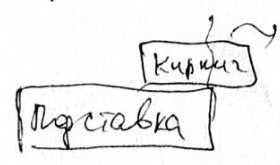
\includegraphics[width=5.2cm]{../figures/lection_1/figure_1.png}
\end{center}
Кирпич, стоящий на подставке --- система в состоянии неустойчивого равновесия. Нас интересует поиск момента фазового перехода (момента, когда кирпич упадёт), точно так же как для плавления, кристаллизации, таяния и других примеров систем. В теории динамических систем это называют точкой бифуркации. Если мы найдём $\varepsilon$-решение, оно не подойдёт, так как нужно, чтобы произошёл <<переход через ноль>>, иначе решение не будет представлять ценности. Может быть найдена не одна точка $x^*$, а интервал.
\paragraph{Определение (точка перехода через ноль в одномерном случае):} $x^*$ --- \textbf{точка перехода через ноль} для $f\in C(\mathbb{R})$, если $\forall \varepsilon > 0 \  f(x^*-\varepsilon)f(x^*+\varepsilon) < 0$.
\subsection{Переход через ноль в многомерном случае}
Пусть $M \subset \mathbb{R}^n$.
\paragraph{Определение (векторное поле):} $\varphi:M\rightarrow\mathbb{R}^n$ --- \textbf{векторное поле}.
\paragraph{Определение (особая точка):} $\mathbf{x^*}$ --- \textbf{особая точка}, если $\varphi(\mathbf{x^*})=\mathbf{0}$.
\paragraph{Определение (изолированная особая точка):} Особая точка $\mathbf{x^*}$ --- \textbf{изолированная}, если $\exists \delta > 0 \  \forall \mathbf{x'}: (\vert\mathbf{x^*}-\mathbf{x'}\vert<\delta \implies \mathbf{x'}$ --- не особая).
\paragraph{Определение (устойчивая особая точка):} Особая точка называется \textbf{устойчивой}, если $\forall \delta > 0 \ \exists \tau > 0$: сдвиг поля на $\delta$ сдвинет особую точку не более, чем на $\tau$.
\\

Задача: найти устойчивые особые точки.
Введём характеристику, которая поможет найти переход через ноль.
Пусть $D \subset \mathbb{R}^n$ --- ограниченное. $\partial D$ --- граница этого множества. $\varphi$ --- невырожденное на $\partial D$ (т.е. нет особых точек).
Пусть $\mathbf{x}=(x_1,x_2,\hdots,x_n) \in \partial D$. Зададим параметризацию границы.
\[
\left\{
\begin{aligned}
x_1 &= x_1(u_1, u_2, \dots, u_{n-1}) \\
x_2 &= x_2(u_1, u_2, \dots, u_{n-1}) \\
&\hdots \\
x_n &= x_n(u_1, u_2, \dots, u_{n-1})
\end{aligned}
\right.
\]
\paragraph{Пример (параметризация границы сферы):} $\left\{
\begin{aligned}
x &= \rho \cos(\psi) \cos(\theta) \\
y &= \rho \cos(\psi) \sin(\theta) \\
z &= \rho \sin(\psi)
\end{aligned}
\right.$
\\

Пусть $S_n$ --- площадь поверхности единичной сферы в $\mathbb{R}^n$.
\[
\gamma(\varphi, \partial D) = \frac{1}{S_n} \int\limits_{\partial D} \frac{1}{\|\varphi(\mathbf{x})\|^n} \begin{vmatrix} \varphi_1(\mathbf{x}) & \frac{\partial \varphi_1(\mathbf{x}}{\partial u_1}  &\hdots & \frac{\partial \varphi_1(\mathbf{x}}{\partial u_{n-1}} \\ \varphi_2(\mathbf{x}) & \frac{\partial \varphi_2(\mathbf{x}}{\partial u_1}  &\hdots & \frac{\partial \varphi_2(\mathbf{x}}{\partial u_{n-1}} \\ \hdots & \hdots & \hdots & \hdots \\ \varphi_n(\mathbf{x}) & \frac{\partial \varphi_n(\mathbf{x}}{\partial u_1}  &\hdots & \frac{\partial \varphi_n(\mathbf{x}}{\partial u_{n-1}} \end{vmatrix} du_1du_2\hdots du_n
\]
\paragraph{Определение (вращение векторного поля по границе):} Величина $\gamma(\varphi, \partial D)$ называется \textbf{вращением векторного поля $\varphi$ по границе $\partial D$}.
\paragraph{Упражнение:} Почему это называется вращением? Подсказка: рассмотрите двумерный случай, простое векторное поле $\varphi(\mathbf{x}) = \mathbf{x}$ и множество $D$ с границей, являющейся окружностью. Показать, что в двумерном случае это количество оборотов вектора поля при движении точки аргумента в положительном направлении по области границы.
\paragraph{Утверджение:} $\mathbf{x^*}$ --- изолированная особая точка, $S_1, S_2$ --- малые сферы вокруг $\mathbf{x^*}$. Тогда верно $\gamma(\mathbf{x^*}, \partial S_1) = \gamma(\mathbf{x^*}, \partial S_2) \implies ind(\mathbf{x^*}) := \gamma(\mathbf{x^*}, \partial S_i) \ \forall i$ --- \textbf{индекс особой точки}.
\paragraph{Теорема:} Изолированная особая точка устойчива $\iff$ $ind(\mathbf{x}) \neq 0$.
\paragraph{Упражнение:} Показать, что особая точка решения квадратного уравнения $x^2+px+q=0$ при $p^2=4q$ не обладает устойчивостью.
\subsection{Метод Чебышёва}
\subsubsection{Постановка задачи}
Решить $F(\mathbf{x}) = 0 \implies$ найти $\mathbf{x^*}: \|F(\mathbf{x^*})\|<\varepsilon, ind(\mathbf{x^*}) \neq 0$.
Если интересуют все решения, то нужно найти множество $\varepsilon$-решений и границы интервалов ненулевого индекса.
Когда ищем так, о перечисленных проблемах 1.2.1 - 1.2.3 думать не нужно.
\subsubsection{Условия метода}
$F(x)=0; F \in C[a; b]; F(a)F(b) < 0 \implies \exists x^* \in [a; b]: F(x^*)=0$ (по т. Больцано-Коши).

Дополнительные ограничения:
\begin{enumerate}
    \item $\forall x \in [a; b]\ \left| F'(x) \right| \ge \delta > 0 \implies \exists \varphi = F^{-1}$ и $\varphi$ имеет столько же непрерывных производных, сколько и $F$. (т. об обратном отображении)
    \item $F$ имеет $(m+1)$ непрерывных производных, $m = const$ (сильное требование!)
\end{enumerate}
\subsubsection{Процедура метода}
\[
x^* \text{ --- решение } \implies F(x^*) = 0 \implies x^* = \varphi(0).
\]

Пусть $x_0$ --- произвольная фиксированная точка. $y_0 = F(x_0)$, $\hat{y}$ --- между $y$ и $y_0$.

По формуле Тейлора
\[
\varphi(y) = \sum\limits_{k = 0}^m \frac{1}{k!} \frac{\partial^k \varphi(y_0)}{\partial y^k} (y-y_0)^k + \frac{1}{(m+1)!}\frac{\partial^{m+1}\varphi(\hat{y})}{\partial y^{m+1}}(y-y_0)^{m+1}.
\]

Пусть $y=0$. Тогда
\[
x^* = \varphi(y_0) + \sum\limits_{k = 1}^m \frac{1}{k!} \frac{\partial^k \varphi(y_0)}{\partial y^k}(-y_0)^k + r_{m+1}(y_0).
\]

\[
x^* = x_0 + \sum\limits_{k = 1}^m \frac{1}{k!} \frac{\partial^k \varphi(y_0)}{\partial y^k}(-y_0)^k + r_{m+1}(y_0).
\]

Пусть $x_1 = x^* - r_{m+1}(y_0)$.

Пусть $y_1 = F(x_1)$.

Применим снова формулу Тейлора в окрестности $y_1$.
\[
x^* = x_1 + \sum\limits_{k=1}^m \frac{1}{k!}\frac{\partial^k\varphi(F(x_1))}{\partial y^k}((-F(x_1))^k) + r_{m+1}(y_1).
\]

Пусть $x_2 = x^* - r_{m+1}(y_1)$.

Пусть $y_2 = F(x_2)$.

Понятно, что $\vert x^* - x_{n}\vert \leq \vert r_{m+1}(y_1) \vert$.


Надежда (увы, это не всегда так):
\begin{enumerate}
    \item $x_n \in [a; b]$
    \item $x_n \underset{n \to \infty}{\longrightarrow} x^*$
\end{enumerate}

Как считать $\frac{\partial^k \varphi(F(x_i))}{\partial y^k}$?
\begin{enumerate}
    \item $y=F(x)$. $\varphi(F(x)) = x$. $\varphi'_y (F(x))F'(x) = 1 \implies \frac{\partial \varphi (F(x))}{\partial y} = \frac{1}{F'(x)}$, $F'(x)$ отдалена от нуля
    \item $\frac{d}{dx}[\varphi'_y (F(x))F'(x)] = 0$. $\varphi'_y (F(x))(F'(x))^2 + \varphi'_y (F(x))F''(x) = 0 \implies \frac {\partial^2 \varphi(F(x))}{\partial^2 y}$ можно выразить: $\varphi''_y (F(x)) = - \frac {\varphi'_y(F(x))F''(x)}{(F'(x))^2}$
\end{enumerate}


На сходимость сложно сформулировать какие-то внятные условия в общем виде.

\subsubsection {Метод Ньютона}
При $m=1$ мы имеем дело с ранее рассмотренным методом Ньютона. 
\[
x_{n+1} = x_n - \frac{F(x_n)}{F'(x_n)}.
\]
Метод может не сходиться, но иногда работает.
\begin{center}
    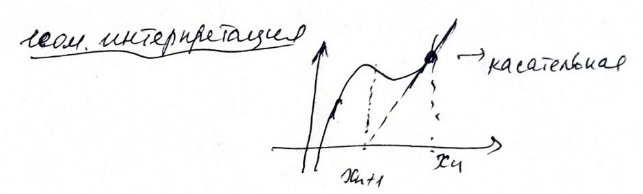
\includegraphics[width=8.2cm]{../figures/lection_1/figure_2.png}
\end{center}